\subsection{Bunch Length}

Bunch length was measured either directly with streak cameras or 
by RF phase scans and observation of beam profile.
RF power levels produced by the PETS gave acces to the effective bunch form-factor,
wich was used to crosscheck the measurements. 

\subsubsection{Streak Camera Measurements }

Streak cameras measured either the emitted synchrotron light or 
transition radiation of an intercepted screens. 

\subsubsection{\label{sec:rfphasescans}RF phase scans}


To ease the discussion, Figure~\ref{fig:PhScans_RF} shows an ideal cos-like accelerating voltage 
on which a bunch is occupying some phase length $\delta \phi$.
%
\begin{figure}[h]
\centering
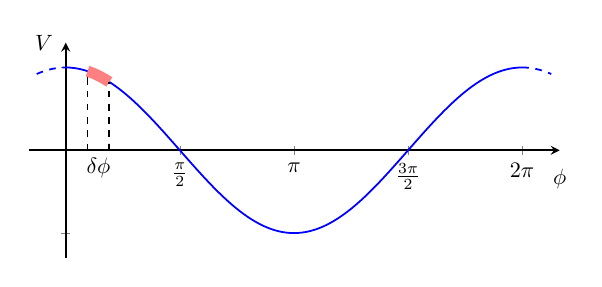
\begin{tikzpicture}[ 
    scale			= 0.8,
    %axis/.style		= {help lines, -{Stealth[length = 1.5ex]}},
    >=stealth
  ]
  \begin{axis}[
       thick,
       axis lines=middle,
       width = 10cm,
       height=5cm,
       xmin = -0.5,
       xmax = 6.8,
       ymin = -1.3,
       ymax = 1.3,
       xtick={0,1.5708,3.14159,4.7123889,6.283},
       xticklabels={$0$,$\frac{\pi}{2}$,$\pi$,$\frac{3\pi}{2}$, $2\pi$},
       yticklabel=\empty,
       x label style={at={(axis description cs:1,0.45)},anchor=north},
       y label style={at={(axis description cs:-0.005,1)},anchor=west},
       axis line style={->},
       xlabel=$\phi$,
       ylabel=$V$,
       domain=0:2*pi
       ]
    \addplot [samples=100,  thick, color=blue]{cos(deg(x))};
    \addplot [domain=-0.4:0, thick, color=blue, dashed]{cos(deg(x))};
    \addplot [domain=2*pi:(2*pi+0.4), thick, color=blue, dashed]{cos(deg(x))};
    \addplot [domain=0.3:0.6, line width=5pt, color=red!50]{cos(deg(x))};
    \addplot [thick, samples=50, smooth,domain=0:2,black, dashed] coordinates {(0.3,0)(0.3,{cos(deg(0.3))})};
    \addplot [thick, samples=50, smooth,domain=0:2,black, dashed] coordinates {(0.6,0)(0.6,{cos(deg(0.6))})};
    \node[below] at (axis cs:0.45, 0) {$\delta \phi$};
   % \legend{$\sin(x)$,$\cos(x)$,$x^2$}
    \end{axis}
\end{tikzpicture}
\caption{Accelerating voltage as a function of phase. In red is depicted a possible bunch of length $\delta \phi$ being accelerated.}
\label{fig:PhScans_RF}
\end{figure}
%
Assuming an ultra-relativistic beam, the beam energy ($E$) after going through 
a single accelerating structure can be written as:
%
\begin{align}
E &= E_0 + \Delta E_{max} \cos(\phi) 
\label{eq:EnergyGain}
\end{align}
%
where $E_0$ is the incoming beam energy; ($\phi = \phi_{RF} - \phi_{beam}$) is 
the phase of the RF ($\phi_{RF}$) with respect to the arrival phase of the beam 
($\phi_{beam}$); $\delta \phi$ is the length of the bunch in phase (see Fig.~\ref{fig:PhScans_RF}); 
$\Delta E_{max}$ is the maximum energy gain which is a constant that depends on 
the power delivered to the accelerating structure and the properties of the structure itself.

If the beam is off-crest in the accelerating structure one would expect, in very first approximation, 
a contribution to energy spread ($\Delta \delta E$) that depends on the bunch length $\delta \phi$ and 
phase $\phi$ equal to:
%
\begin{align}
\Delta \delta E &\approx \Delta E_{max} \sin(\phi) \delta \phi
\label{eq:energySpreadIncreaseBase}
\end{align}
%
In the limit case of $\phi = 0$ one gets maximum acceleration and, in first approximation, 
no energy spread variation.
In this case one might still want to estimate the impact on energy spread, 
which could be computed as:
%
\begin{align}
\Delta \delta E &= E_{max} \left(1-\cos\left(\frac{\delta \phi}{2}\right)\right).
\label{eq:energySpreadIncreaseOnCrest}
\end{align} 


%
The contribution from Eq.~(\ref{eq:energySpreadIncreaseBase}) should then be added in quadrature 
to the initial beam energy spread ($\delta E_0$).
%
In reality, the incoming beam might have some time-correlated energy spread, 
therefore a more precise estimation of the final beam energy spread is:
%
\begin{align}
\delta E &= \sqrt{
(\delta E_0)^2 + 
\left(
C
+
\Delta E_{max} \sin(\phi)
\right)^2  \delta\phi ^2
}
\label{eq:completeEnergySpreadVariation}
\end{align}
%
where $\delta E_0$ is the initial \emph{un-correlated} energy spread, 
$C$ is the incoming beam energy-spread-time correlation factor.

%
By doing a scan of $\phi_{RF}$ and by measuring the final energy $E$, 
from Eq.~(\ref{eq:EnergyGain}) one can fit $E_0$,  $\Delta E_{max}$ and beam phase $\phi_{beam}$.
%
At the same time, by rerecording also the beam energy spread variation, 
one can fit Eq.~(\ref{eq:completeEnergySpreadVariation}) unknown parameters: 
$\delta E_0$, $C$ and the sought $\delta\phi$.

Note that $\delta\phi$ is in units of $2 \pi$. The bunch length in seconds ($\delta\phi_{s}$) is 
linked to the RF frequency ($f_{RF}$) via:
%
\begin{align}
\delta\phi_{s} &= \frac{1}{f_{RF}} \frac{\delta\phi}{2 \pi}
\label{eq:conversionRadToS}
\end{align}
%

The above equations can be used only assuming Gaussian distributions, 
for which $\delta\phi$, $\delta E_0$, $\Delta \delta E$ can either be, consistently, 
the r.m.s. or FWHM values using the known relation:
\begin{align}
{\mathrm  {FWHM}}=2{\sqrt  {2\ln 2}}\;\sigma \approx 2.355\;\sigma.
\end{align}



% Assuming an ultra-relativistic electron beam, and dealing with only one accelerating structure, 
% one would expect that the acceleration and energy spread variation goes like:
% %
% \begin{align}
% \Delta E &= A \cos(\phi) \label{eq:energyIncreaseBase} \\
% \Delta \delta E &= A \sin(\phi) \delta \phi \label{eq:energySpreadIncreaseBase}
% \end{align}
% %
% where $\phi$ is the phase of the beam respect to the RF; 
% $\delta \phi$ is the length of the bunch in phase; 
% $A$ is some constant that depends on the power delivered to 
% the accelerating structure and the properties of the structure itself.
% Clearly if $\phi = 0$ one gets maximum acceleration and, in first approximation, 
% no energy spread variation. If $\phi = \pi/2$ the effect is opposite.
% 
% If one starts from a beam that has already some energy and energy spread ($E_0$ and $\delta E_0$) and 
% assuming that the bunch length is constant over the whole process, one gets as final energy:
% %
% %
% \begin{align}
% E &= E_0 + A \cos(\phi) \\
% \delta E &= \sqrt{(\delta E_0)^2 + (A \sin(\phi) \delta \phi )^2} \label{eq:sumEnergySpreadsQuadrature}
% \end{align}
% %
% where we added in quadrature the energy spreads. 
% The sum in quadrature is a reasonable assumption, even if not formally correct: 
% the initial energy spread and the additional energy spread gained during 
% the acceleration are a priori not independent.
% In the worst case one can replace eq.~\ref{eq:sumEnergySpreadsQuadrature} with a direct sum:
% %
% \begin{align}
% \delta E &= \delta E_0 + A \sin(\phi) \delta \phi  \label{eq:sumEnergySpreadsDirect}
% \end{align}
% %
% 
% An other special case is when the beam bunch is on-crest. 
% Here Eq.~\ref{eq:energySpreadIncreaseBase} is \emph{underestimating} the energy spread increase. 
% In the limit case where $\phi = 0$ one gets $\Delta \delta E = 0$ as well, 
% however a more realistic approximation would be:
% %
% \begin{align}
% \Delta \delta E &= A \left(1-\cos\left(\frac{\delta \phi}{2}\right)\right)\label{eq:energySpreadIncreaseOnCrest}
% \end{align}
% % 
% 
